\chapter{Interaksi Basisdata}
\section{MySQL}
%create user: create user 'arya'@'localhost' identified by '123456';
%create database: create database iris;
%grant user: grant all on 'iris.* to 'arya'@'localhost';
%flush privileges;
%create table irisdata (sepallength real(2,1), sepalwidth real(2,1), petallength real(2,1), petalwidth real(2,1), kelas varachr(15));
Modifikasi \lstlistingname~\ref{lst:bacairis} sehingga menjadi seperti \lstlistingname~\ref{lst:insertiris}. Hasil ekseksinya ditunjukkan \figurename~\ref{fig:insertmysql}.
 
\lstinputlisting[language=python, numbers=left, numberstyle=\small, caption=Membaca dataset iris dan menyimpannya di MySQL, showstringspaces=false, label=lst:insertiris]{script/insertiris.py} 

\begin{figure}
  \begin{center}
    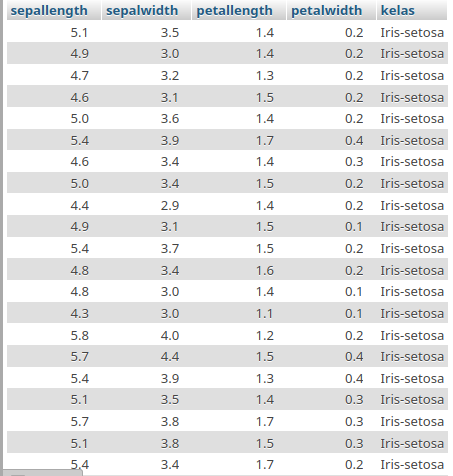
\includegraphics[scale=2.0]{pics/insertmysql.png}
    \caption{Hasil dari proses memasukkan data ke server MySQL}
    \label{fig:insertmysql}
  \end{center}
\end{figure}
\section{PostgreSQL}
Modifikasi \lstlistingname~\ref{lst:insertiris} sehingga menjadi seperti \lstlistingname~\ref{lst:insertirispg}. Hasil ekseksinya ditunjukkan \figurename~\ref{fig:insertpgsql}.

\lstinputlisting[language=python, numbers=left, numberstyle=\small, caption=Membaca dataset iris dan menyimpannya di pgSQL, showstringspaces=false, label=lst:insertirispg]{script/insertirispg.py}

\begin{figure}
  \begin{center}
    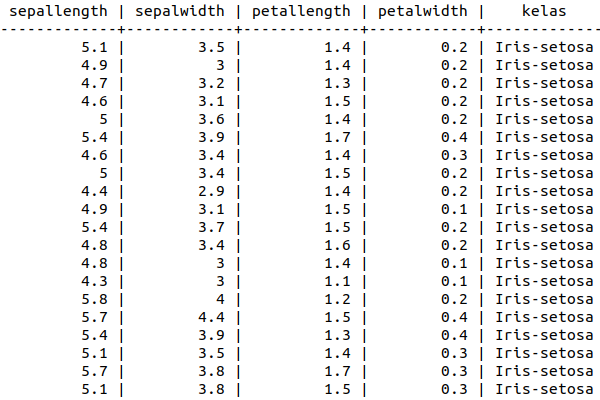
\includegraphics[scale=2.0]{pics/insertpgsql.png}
    \caption{Hasil dari proses memasukkan data ke server pgSQL}
    \label{fig:insertpgsql}
  \end{center}
\end{figure}

%https://computingforgeeks.com/installing-postgresql-database-server-on-ubuntu/
%https://linuxhint.com/postgresql_installation_guide_ubuntu_20-04/
%https://www.howtoforge.com/tutorial/ubuntu-postgresql-installation/
\section{MongoDB}
MongoDB adalah salah satu basisdata non-relasional yang menyimpan data berbasis dokumen. Bukan dokumen seperti berkas yang digunakan pengolah teks seperti Microsoft Word$\copyright$, tetapi JSON (\textit{JavaScript Object Notation}) seperti dilustrasikan \figurename~\ref{fig:jsonmongo}\footnote{\url{https://www.mongodb.com/blog/post/getting-started-with-python-and-mongodb}}.

\begin{figure}
  \begin{center}
    \includegraphics[scale=.75]{pics/JSONExamplePythonMongoDB.png}
    \caption{Ilustrasi penyimpanan data berbasis dokumen oleh MongoDB}
    \label{fig:jsonmongo}
  \end{center}
\end{figure}

Sedangkan \tablename~\ref{tab:relasimongo} menunjukkan perbandingan konsep pada basisdata relasional terhadap basisdata non-relasional seperti MongoDB\footnote{\url{https://www.mongodb.com/blog/post/getting-started-with-python-and-mongodb}}.

\begin{table}[h]
\caption{Komparasi konsep basisdata relasional vs. non-relasional}
\label{tab:relasimongo}
  \begin{center}
    \begin{tabular}{@{}cc@{}}\toprule
    %\hline
    Relasional & Non-relasional\\ \midrule
  \textit{Database} & \textit{Database} \\ 
  \textit{Table} & \textit{Collection} \\
  \textit{Rows} & \textit{Documents}\\
  \textit{Index} & \textit{Index}\\
       \bottomrule
    \end{tabular}
  \end{center}
\end{table}

Sebagai bahan latihan, kita akan menggunakan dataset yang digunakan dalam artikel \cite{peerreview}\footnote{\url{https://github.com/allenai/PeerRead}}. Perhatikan \lstlistingname~\ref{lst:readjson} yang bertujuan untuk mengeksplorasi struktur berkas json secara rekursif. Dari \lstlistingname~\ref{lst:readjson} kita dapat mengambil pasangan \textit{key}-\textit{value} dari struktur berkas json.

\lstinputlisting[language=python, numbers=left, numberstyle=\small, caption=Mengeksplorasi struktur berkas json, showstringspaces=false, label=lst:readjson]{script/readjson.py}

Setelah berhasil melakukan pembacaan berkas json, sekarang saatnya mencoba memasukkan data berkas json ke MongoDB. Perhatikan \lstlistingname~\ref{lst:savejson}.

\lstinputlisting[language=python, numbers=left, numberstyle=\small, caption=Menyimpan berkas json ke MongoDB, showstringspaces=false, label=lst:savejson]{script/savemongo.py}

 


%https://www.geeksforgeeks.org/how-to-import-json-file-in-mongodb-using-python/
%https://www.w3schools.com/python/python_mongodb_getstarted.asp
%https://www.programiz.com/python-programming/json
%https://www.geeksforgeeks.org/python-mongodb-query/?ref=rp
